\documentclass{article}

% Provisional layout test using the official ICASSP 2026 kit. Replace the kit
% with the official ICASSP 2027 submission files when they become available.
\usepackage{spconf,amsmath,graphicx,hyperref}
\usepackage{booktabs,url}
\hypersetup{hidelinks}

\graphicspath{{../figures/}}
\newcommand{\deltanll}{\Delta(-\mathrm{NLL})}

\title{Does Clinical Metadata Alignment Transfer Disease Evidence? A
Pairing-Controlled Audit of Respiratory Audio under Cohort Shift}

\name{Author names withheld in this layout test}
\address{Affiliations to be inserted before submission}

\begin{document}
\ninept
\maketitle

\begin{abstract}
Clinical audio models increasingly align recordings with clinical metadata, although
symptoms and demographics may encode cohort construction rather than audible evidence. We
test whether alignment learns participant correspondence or disease evidence that transfers
across populations. Frozen AST-6L and Phi-2 encoders are connected by a RespiraMFM-style
projector trained with correct metadata, metadata shuffled within COVID label, or globally
shuffled. Within-label shuffling preserves label-level co-occurrence while removing
individual correspondence. In UKCOVID, recruitment source predicts COVID with AUROC 0.9966
in training but 0.5000 after covariate matching. Correct pairing improves source AUROC over
within-label shuffling (+0.0140 [0.0040, 0.0235]) yet worsens matched negative
log-likelihood ($\deltanll=-0.0249$ [-0.0443, -0.0069]); its matched AUROC difference is
uncertain (+0.0062 [-0.0144, 0.0279]). Probes confirm learned participant correspondence,
especially sex, without transferable disease benefit. OPERA-CT repeats the negative
matched NLL direction. These results motivate within-label controls and covariate-balanced
evaluation for clinical audio--metadata alignment.
\end{abstract}

\begin{keywords}
respiratory audio, contrastive learning, clinical metadata, cohort shift, confounding
\end{keywords}

\section{Introduction}
Clinical audio models often use symptoms, demographics, medical history, or text assembled
from those fields. Contrastive alignment can make this context accessible to an audio
representation \cite{siam2026respiramfm}. Yet, unlike an audible description of pitch or
timing, clinical metadata may describe the participant or recruitment process rather than
the waveform. A model can therefore learn the intended mapping while exploiting cohort
structure that does not transfer.

UKCOVID makes this ambiguity measurable. Its Standard training distribution combines a
largely positive Test-and-Trace cohort with a largely negative population-surveillance
cohort. Recruitment source alone predicts COVID with AUROC 0.9966 in Standard train but
0.5000 in the covariate-matched test population. Symptoms are also a strong recruitment
proxy: ``no symptoms'' occurs in 0.786 of training negatives and 0.019 of positives.
Aligning audio to symptom text may thus reinforce a source-specific association
\cite{coppock2024audio}.

A global shuffle cannot isolate this mechanism because it removes both participant
correspondence and disease-level co-occurrence. We introduce a \emph{within-label shuffle}:
each recording is paired with another same-label participant's metadata. Correct and
within-label arms share label-level statistics and differ only in individual pairing.

Our contributions are: (i) a pairing-controlled protocol separating participant
correspondence from label-level audio--metadata co-occurrence; (ii) a transfer audit using
source and covariate-matched populations, with calibrated NLL as the primary outcome; and
(iii) direct-fusion, second-backbone, and probe controls separating weak audio increment
from alignment-specific effects and learned participant mapping.

\begin{figure*}[t]
  \centering
  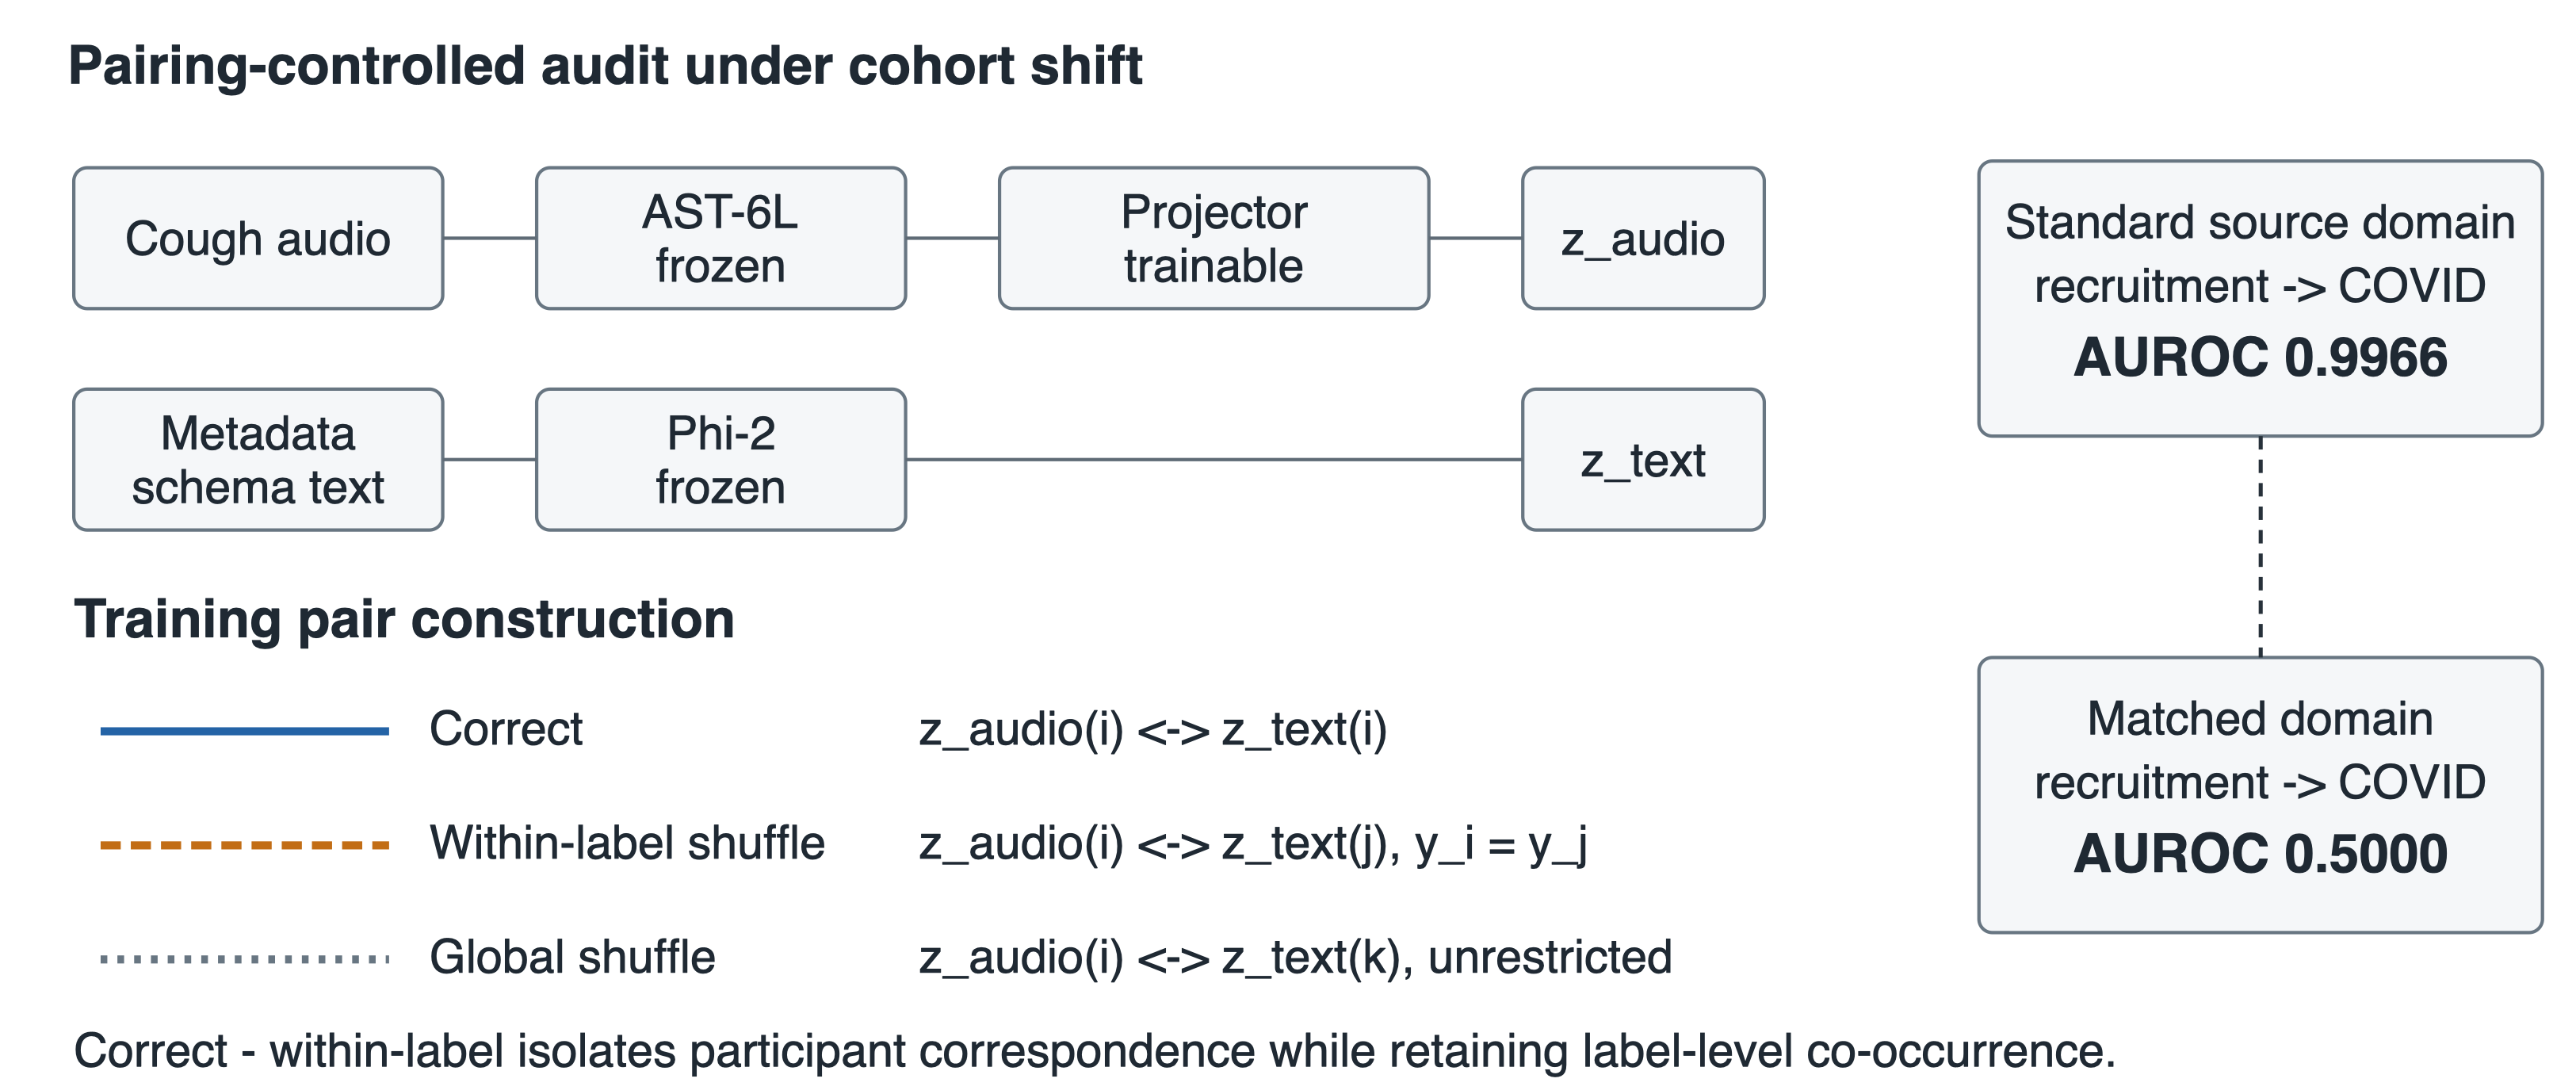
\includegraphics[width=\textwidth]{icassp_pairing_design.png}
  \caption{Pairing-controlled training and evaluation under cohort shift. Correct and
  within-label arms preserve the same COVID-label co-occurrence.}
  \label{fig:design}
\end{figure*}

\section{Method}
\subsection{Data and representations}
We learn representations on the patient-level UKCOVID Standard train split
\cite{budd2024ukcovid}. After the frozen audio-availability audit, it contains 20,714
participants. We evaluate Standard, the primary covariate-matched test set, and the
participant-disjoint matched-long sensitivity set. Because official tests informed earlier
protocol development, these results are a \emph{discovery audit}, not independent
confirmation.

Audio is encoded by frozen six-layer Audio Spectrogram Transformer features
\cite{gong2021ast}; text is encoded by frozen Phi-2 \cite{javaheripi2023phi2}. Metadata is
deterministically rendered from age, sex, smoking, asthma, other respiratory conditions,
and symptoms, with missingness explicit. COVID results, test details, recruitment source,
timestamps, and recording artefacts are excluded.

Only an audio-side projector is trained, following RespiraMFM Stage 1
\cite{siam2026respiramfm}. It maps 768 to 1,024 to 2,560 dimensions using LayerNorm and ReLU
after both linear layers and dropout 0.1 after the first. For frozen audio embedding $a_i$,
frozen text embedding $t_i$, and projector $f_\theta$, the one-directional objective is
\begin{equation}
\mathcal{L}=-\frac{1}{N}\sum_i\log
\frac{\exp(\bar f_\theta(a_i)^\top\bar t_i/\tau)}
{\sum_j\exp(\bar f_\theta(a_i)^\top\bar t_j/\tau)},\quad\tau=0.07,
\end{equation}
where bars denote $\ell_2$ normalization inside the loss. The primary downstream
representation is the raw post-ReLU output; $\ell_2$-normalized output is a prespecified
sensitivity.

\subsection{Pairing arms and evaluation}
The trained arms are \emph{correct}, \emph{within-label shuffled}, and \emph{globally
shuffled}. Within each of five seeds, they share initialization, audio batch order, and
dropout stream; only pairing differs. A shuffled mapping is sampled once per seed, forbids
self-pairs, and remains fixed for 500 epochs. We use batch size 64 and Adam at $10^{-3}$,
with no scheduler or weight decay. All 15 projector runs completed, and only their final
checkpoints are evaluated. Raw frozen AST is the unaligned reference. This is a Stage-1
reimplementation, not a reproduction of the full Phi-2/LoRA system.

All representations use the same regularized logistic readout. Regularization is selected
per seed on complete Standard validation, where a source-domain Platt calibrator is also
fit. Matched results select no parameter. The preregistered primary comparison is correct
minus within-label on matched, measured as paired $\deltanll$; positive values favour
correct pairing. AUROC is secondary. Intervals hierarchically resample participants and
seeds while retaining paired arm predictions. Linear probes measure decodability, not
causal classifier use.

As an attribution control, we concatenate the same schema metadata with raw AST under the
same linear protocol. A prespecified robustness analysis repeats the full alignment
experiment with frozen OPERA-CT respiratory-audio features \cite{zhang2024opera}, changing
only the backbone.

\subsection{External stress test}
Before any external model score, we froze a Coswara v1.0 protocol
\cite{bhattacharya2023coswara} using one cough-heavy recording per participant, objective
waveform QC, decoded-PCM duplicate control, patient-disjoint development splits, and 1:1
covariate matching. Formal execution required at least 100 pairs, maximum absolute SMD
0.12, maximum fine-balance difference 0.08, and adequate development class counts. We
extracted all 2,746 recordings; 2,646 passed objective QC. Exact matching yielded at most
112 pairs. Frozen trimming reached the 100-pair floor with maximum categorical SMD 0.140,
so the gate failed. No Coswara representation, classifier, or model score was produced.

\begin{figure*}[t]
  \centering
  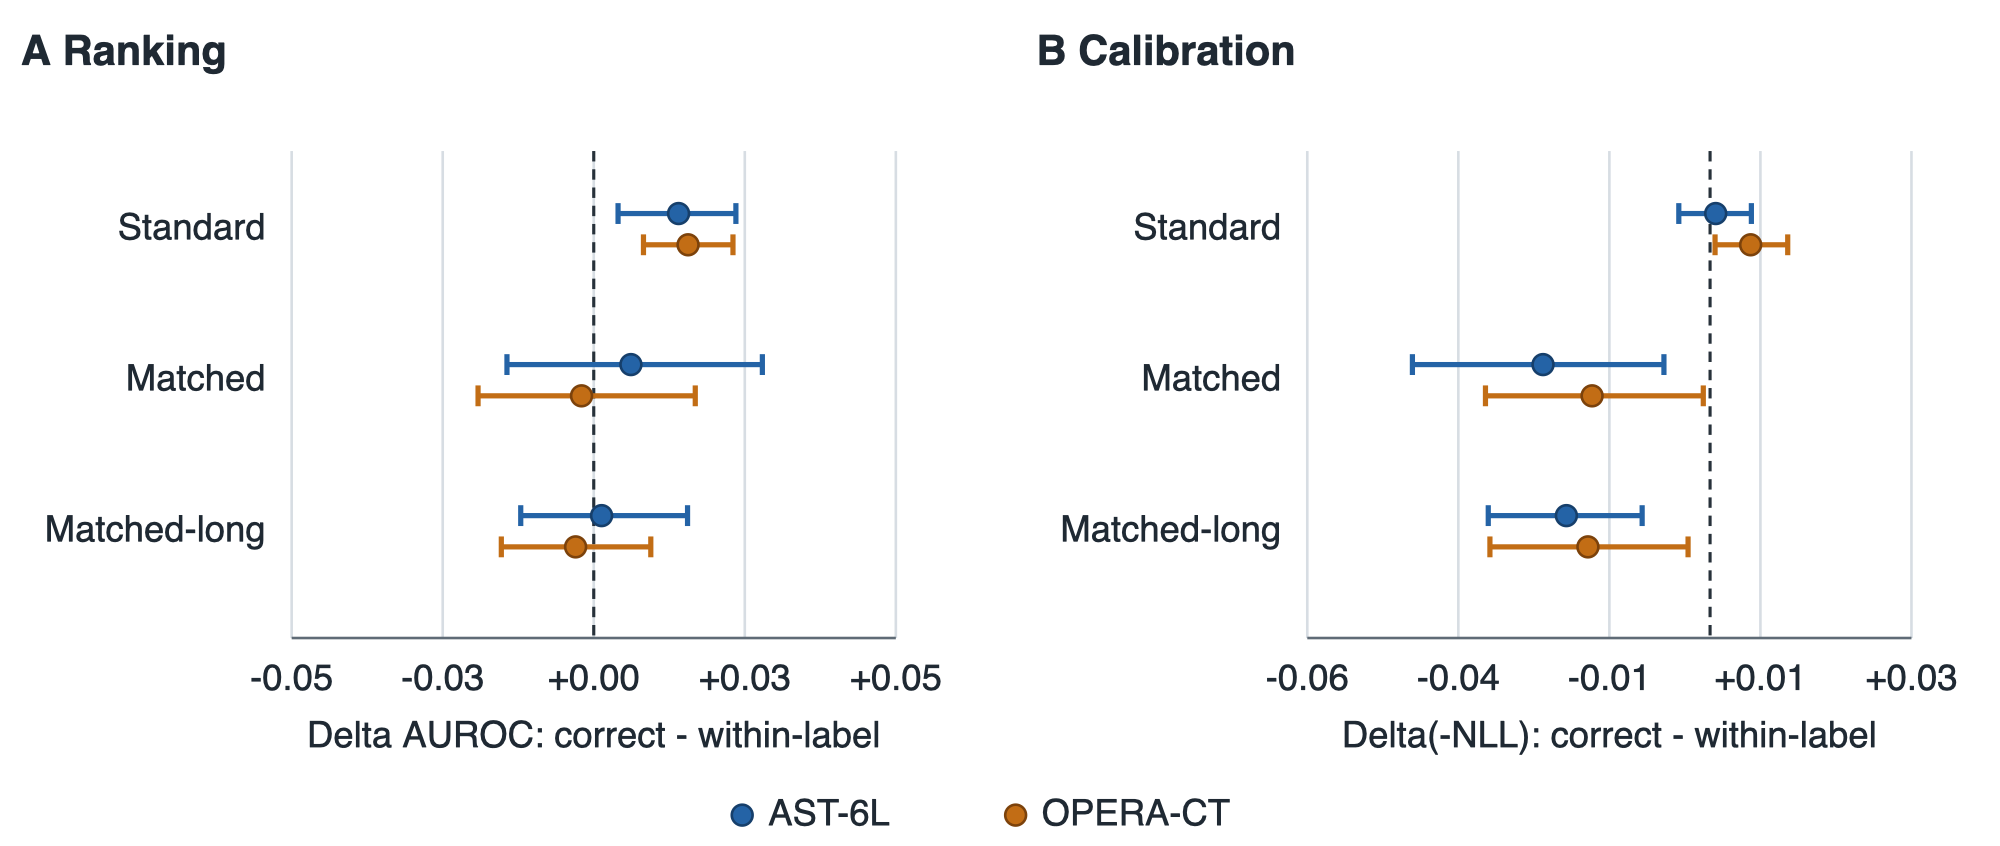
\includegraphics[width=\textwidth]{icassp_pairing_forest.png}
  \caption{Correct-minus-within-label $\Delta$AUROC (left) and $\deltanll$ (right) for
  AST-6L and OPERA-CT across Standard, matched, and matched-long.}
  \label{fig:paired}
\end{figure*}

\section{Results}
\subsection{Disease transfer}
Table~\ref{tab:absolute} reports absolute performance. Correct exceeds within-label AUROC
in Standard (0.649 versus 0.635). Under matching, aligned representations approach chance
ranking and the globally shuffled projector has lower NLL than the correct projector.
Consequently, correct-versus-raw improvement cannot alone establish semantic alignment:
projection or regularization can change calibration without using correct pairing.

\begin{table}[t]
\centering
\caption{COVID performance as AUROC / NLL (lower NLL is better).}
\label{tab:absolute}
\setlength{\tabcolsep}{3.0pt}
\begin{tabular}{lcccc}
\toprule
 & Raw & Correct & Within & Global \\
\midrule
Standard & .708/.604 & .649/.628 & .635/.628 & .571/.640 \\
Matched & .538/.857 & .529/.795 & .523/.770 & .510/.739 \\
Matched-L & .548/.850 & .532/.794 & .530/.773 & .524/.737 \\
\bottomrule
\end{tabular}
\end{table}

The paired contrast separates source correspondence from matched transfer
(Table~\ref{tab:paired}). Correct pairing gives a detectable Standard AUROC increment of
+0.0140, while its Standard NLL difference is uncertain. On matched, the primary
$\deltanll$ is -0.0249 (95\% CI [-0.0443, -0.0069]); all five seed effects are negative.
Matched AUROC changes by only +0.0062 with an interval crossing zero. Matched-long shows
the same NLL direction and near-zero AUROC difference. Normalization preserves the NLL
direction: normalized matched $\deltanll$ is -0.0179 [-0.0371, 0.0011], and matched-long is
-0.0204 [-0.0328, -0.0082].

This is not solely an alignment-specific failure. On matched, adding raw AST to metadata
gives $\Delta$AUROC +0.0028 [-0.0019, 0.0071] and $\deltanll$ -0.0034 [-0.0194, 0.0126].
Correct alignment also does not improve over metadata plus raw AST
($\Delta$AUROC -0.0040 [-0.0093, 0.0015]; $\deltanll$ -0.0077 [-0.0301, 0.0157]).

OPERA-CT reproduces the prespecified direction. Correct minus within-label is positive in
Standard ($\Delta$AUROC +0.0156 [0.0082, 0.0230]) but negative in matched NLL
($\deltanll$ -0.0176 [-0.0335, -0.0010]); all five seed effects are negative. Its matched
AUROC effect is -0.0020 [-0.0191, 0.0168], and matched-long repeats the negative NLL
(-0.0182 [-0.0328, -0.0033]). Normalization preserves the direction.

\begin{table}[t]
\centering
\caption{Correct minus within-label paired effects [95\% CI].}
\label{tab:paired}
\setlength{\tabcolsep}{3.2pt}
\begin{tabular}{lcc}
\toprule
 & $\deltanll$ & $\Delta$AUROC \\
\midrule
Standard & +.0008 [-.0047,.0062] & +.0140 [.0040,.0235] \\
Matched & -.0249 [-.0443,-.0069] & +.0062 [-.0144,.0279] \\
Matched-L & -.0214 [-.0330,-.0101] & +.0013 [-.0121,.0155] \\
\bottomrule
\end{tabular}
\end{table}

\subsection{What correspondence was learned?}
The correct arm did not simply fail to learn its mapping. On matched, correct minus
within-label probe AUROC is +0.1912 [0.1677, 0.2156] for sex and +0.0465 [0.0069, 0.0854]
for age at least 65. Effects are uncertain for recruitment source (+0.0138 [-0.0205,
0.0473]), cough (+0.0098 [-0.0114, 0.0309]), and no symptoms (+0.0151 [-0.0096, 0.0407]).
Symptoms instead improve mainly between global and within-label arms, consistent with
label-level co-occurrence. Raw AST has higher absolute AUROC than correct alignment on
every probe (e.g., sex 0.871 versus 0.812 and age 0.742 versus 0.657). We therefore infer
selective retention relative to the within-label projector, not demographic information
added beyond raw AST.

\subsection{Coswara status}
The preregistered Coswara gate returned NO-GO before model execution. All 2,746 recordings
decoded, but 100 failed objective QC. At the frozen 100-pair floor, categorical imbalance
remained above threshold (maximum absolute SMD 0.140 versus 0.12). We changed no threshold
or matching field, read no model prediction, and claim no cross-dataset confirmation.

\section{Discussion and Conclusion}
Correct pairing produced both a source-domain ranking gain and strong participant-level sex
correspondence; calling alignment wholly ineffective would therefore be inaccurate.
Nevertheless, the preregistered matched NLL comparison was negative, matched AUROC was
uncertain, matched-long agreed in NLL direction, and OPERA-CT reproduced this pattern. In
this setting, learning genuine clinical metadata correspondence did not guarantee portable
disease evidence.

Within-label shuffling makes this interpretation possible. Unlike global shuffling, it
retains the disease--metadata association and removes only participant identity. It should
accompany global controls whenever cohort metadata is label-associated.

The study does not establish that metadata alignment is universally harmful or that either
backbone contains no COVID information. It tests one Stage-1 projector, two frozen
backbones, and a linear readout in an unusually confounded dataset. UKCOVID is exploratory;
matched-long is not independent replication; probe decodability does not establish causal classifier use;
and the Coswara branch stopped at its preregistered data-feasibility gate. Future work
should use untouched cohorts with sufficient covariate overlap, nonlinear readouts, and
separate audible evidence from independent clinical context.

In summary, correct audio--metadata pairing learns participant correspondence and a small
source-domain ranking advantage, but not improved calibrated disease prediction after
covariate balancing. Clinical audio--metadata studies should minimally include a
within-label shuffle and a cohort-balanced transfer evaluation.

\bibliographystyle{IEEEbib}
\bibliography{references}

\end{document}
